% vim: set textwidth=78 autoindent:

% when the revision of a section has been finalized,
% comment out the following line:
%\updatedisclaimer

\section{Vector Attribute Data}\label{sec:attributes}
\begin{tabular}{p{3.5cm}p{6cm}p{6cm}}
\multirow{2}{*}{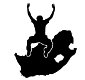
\includegraphics[width=2.5cm]{logo}} & Objectives: &
In this topic we describe how attribute data are associated with vector
features and can be used to symbolise data. \\
& & \\
& Keywords: & 
Attribute, database, fields, data, vector, symbology \\
\hline
\end{tabular}

\subsection{Overview}\label{subsec:overview}

If every line on a map was the same colour, width, thickness, and had the
same label, it would be very hard to make out what was going on. The map
would also give us very little information. Take a look at Figure
\ref{fig:rendercompare} below for example. 

\begin{figure}[ht]
   \begin{center}
   \caption{Maps come to life when colour and different symbols are used to
help you to tell one type of feature from the next. Can you tell the
difference between rivers, roads and contours using the map on the left?
Using the map on the right it is much easier to see the different features.}
\label{fig:rendercompare}\smallskip
   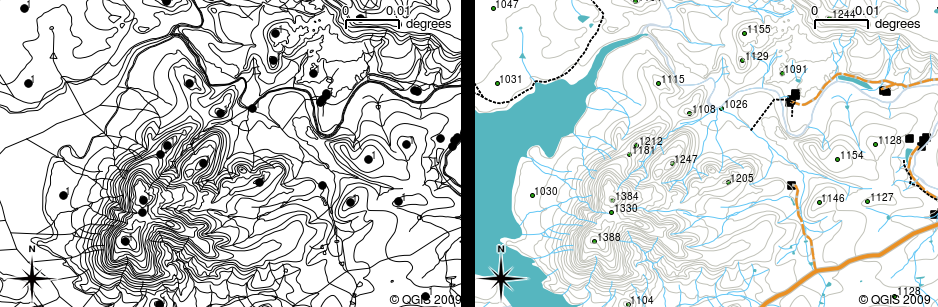
\includegraphics[clip=true, width=\textwidth]{RenderAsComparison}
\end{center}
\end{figure}

In this topic we will look at how attribute data can help us to make
interesting and informative maps. In the previous topic on vector data, we
briefly explained that \textbf{attribute data} are used to \textbf{describe
vector features}. Take a look at the house pictures in Figure
\ref{fig:houses} below.

The geometry of these house features is a polygon (based on the floor plan of
the house), the attributes we have recorded are roof colour, whether there is
a balcony, and the year the house was built. Note that attributes don't have
to be visible things - they can describe things we know about the feature
such as the year it was built. In a GIS Application, we can represent this
feature type in a houses polygon layer, and the attributes in an attribute
table (see Figure \ref{fig:attrtable}).

%% Minipage to put both figures on one page
\begin{figure}[htpb]
   \begin{minipage}[h]{\textwidth}
   \begin{center}
   \caption{Every feature has characteristics that we can describe. These can
be visible things, or things we know about the feature (e.g. year built).}
   \label{fig:houses}\smallskip
   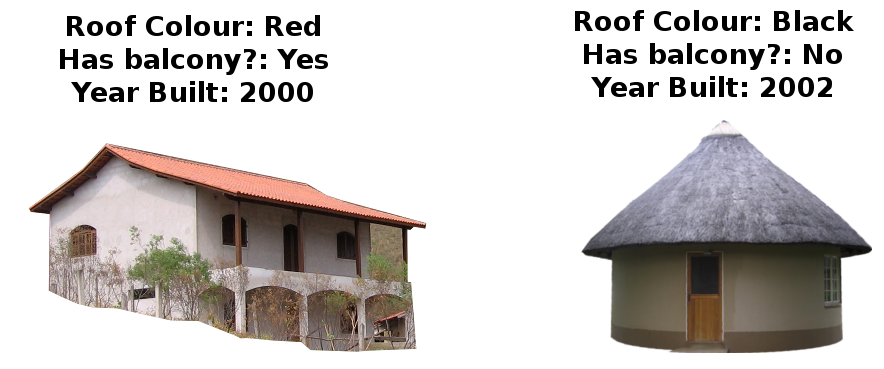
\includegraphics[clip=true, width=0.9\textwidth]{Houses}
   \end{center}
   \end{minipage} \\
   \vspace{1cm}
   \begin{minipage}[h]{\textwidth}
   \begin{center}
   \caption{A houses layer. House features have attributes that describe the
houses' roof colour and other properties. The attribute table (lower image)
lists the attributes for the house areas shown on the map. When a feature is
highlighted  in the table, it will appear as a yellow polygon on the map.}
   \label{fig:attrtable}\smallskip
   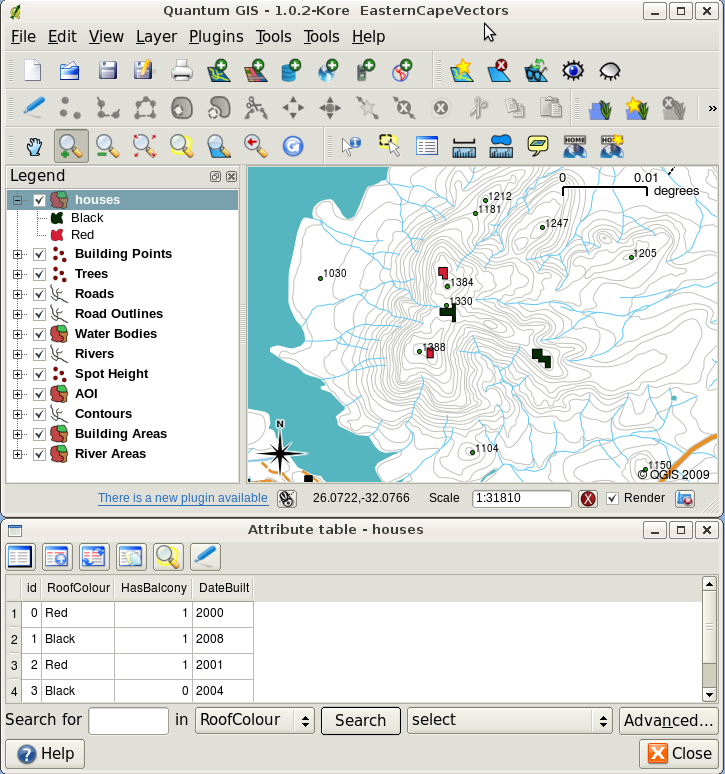
\includegraphics[clip=true, width=0.6\textwidth]{AttributeTable}
   \end{center}
   \end{minipage}
\end{figure}

The fact that features have attributes as well geometry in a GIS Application
opens up many possibilities. For example we can use the attribute values to
tell the GIS what colours and style to use when drawing features (see Figure
\ref{fig:houseroofbalc}). The process of setting colours and drawing styles is
often referred to as setting feature \textbf{symbology}. 

Attribute data can also be useful when creating \textbf{map labels}. Most GIS
Applications will have a facility to select an attribute that should be used
to label each feature. 

\begin{figure}[ht]
   \begin{center}
   \caption{In a GIS Application, we can draw features differently depending
on their attributes. On the left we have drawn house polygons with the same
colour as the roof attribute. On the right we colour coded houses according
to whether they have a balcony or not.}
\label{fig:houseroofbalc}\smallskip
   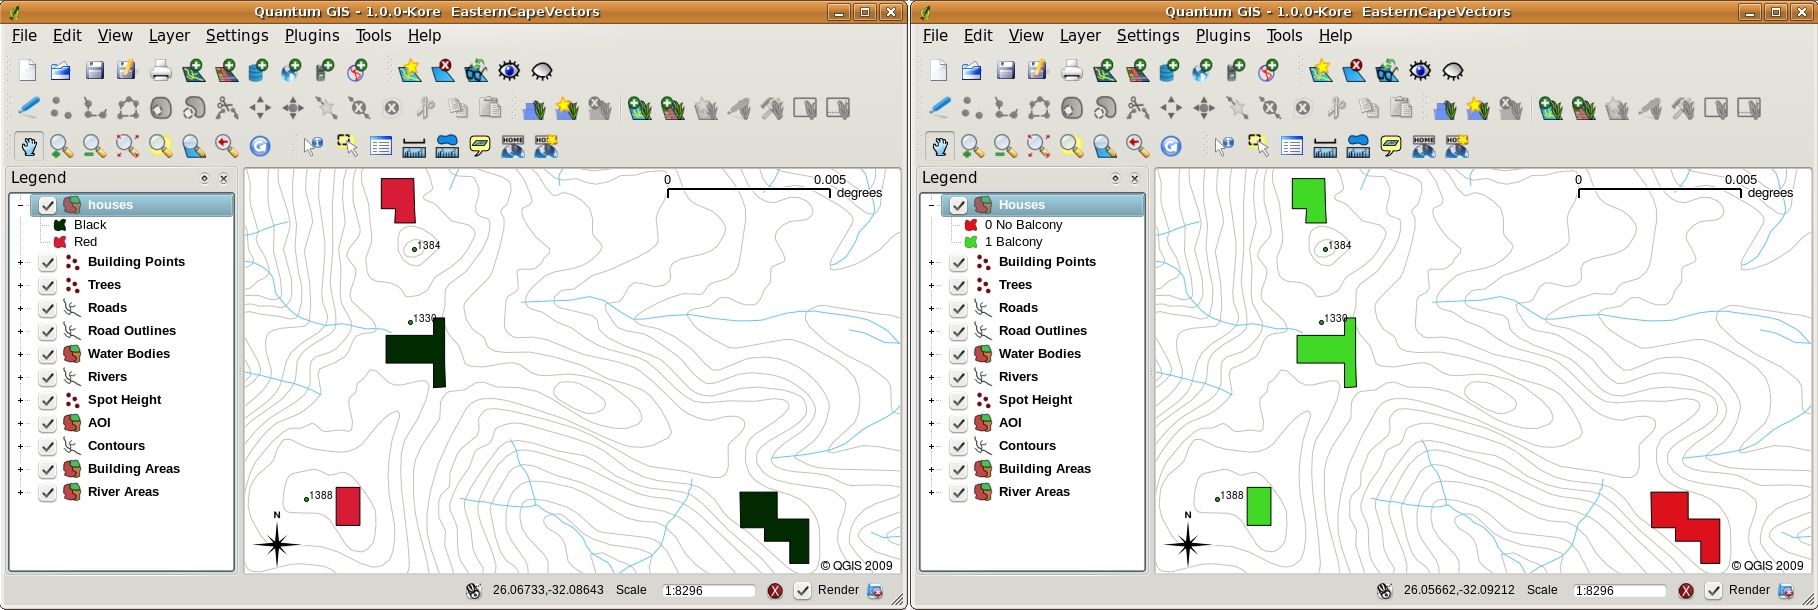
\includegraphics[clip=true, width=\textwidth]{HousesByBalconyRoof}
\end{center}
\end{figure}

If you have ever \textbf{searched a map} for a place name or a specific
feature, you
will know how time consuming it can be. Having attribute data can make
searching for a specific feature quick and easy. In Figure
\ref{fig:housesearch} you can see an example of an attribute search in a GIS. 

Finally, attribute data can be very useful in carrying out \textbf{spatial
analysis}.
Spatial analysis combines the spatial information stored in the geometry of
features with their attribute information. This allows us to study features
and how they relate to each other. There are many types of spatial analysis
that can be carried out, for example, you could use GIS to find out how many
red roofed houses occur in a particular area.  If you have tree features, you
could use GIS to try to find out which species might be affected if a piece
of land is developed. We can use the attributes stored for water samples
along a river course to understand where pollution is entering into the
stream. The possibilities are endless! In a later topic we will be exploring
spatial analysis in more detail.

Before we move on to attribute data in more detail, let's take a quick recap:

Features are real world things such as roads, property boundaries, electrical
substation sites and so on. A \textbf{feature} has a \textbf{geometry} (which
determines if it is a \textbf{point}, \textbf{polyline} or \textbf{polygon})
and \textbf{attributes} (which describe the feature).
This is shown in Figure \ref{fig:attdiagram}. 

%% Minipage to put both figures on one page
\begin{figure}[htpb]
   \begin{minipage}[h]{\textwidth}
   \begin{center}
   \caption{In a GIS Application, we can also search for features based on
their attributes. Here we see a search for houses with black roofs. Results
are shown in yellow in the map, turquoise on the table.}
\label{fig:housesearch}\smallskip
   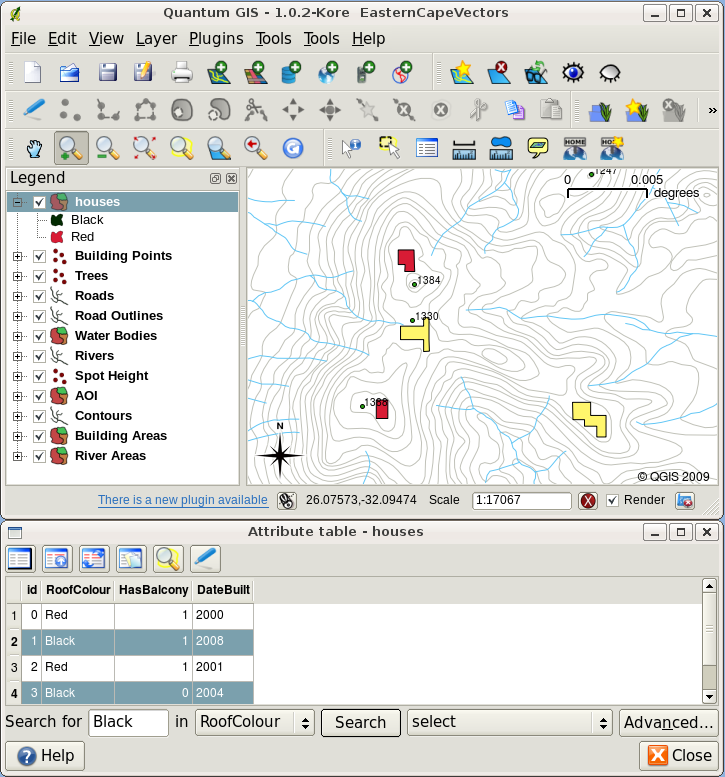
\includegraphics[clip=true, width=0.6\textwidth]{HousesSearch}
   \end{center}
   \end{minipage} \\
   \vspace{1cm}
   \begin{minipage}[h]{\textwidth}
   \begin{center}
   \caption{Vector features at a glance.}
   \label{fig:attdiagram}\smallskip
   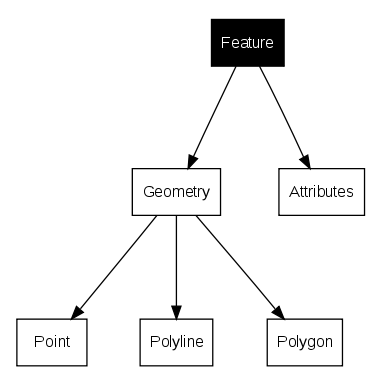
\includegraphics[clip=true, width=0.5\textwidth]{attribute_diagram}
   \end{center}
   \end{minipage}
\end{figure}

\subsection{Attributes in detail}

Attributes for a vector feature are stored in a \textbf{table}. A table is like a
spreadsheet. Each column in the table is called a \textbf{field}. Each row in the
table is a record. Table \ref{tab:attributes} shows a simple example of how
an attribute
table looks in a GIS. The records in the attribute table in a GIS each
correspond to one feature. Usually the information in the attribute table is
stored in some kind of database. The GIS application links the attribute
records with the feature geometry so that you can find records in the table
by selecting features on the map, and find features on the map by selecting
features in the table.

%% Note: xdvi does not show white text on black background but it works!
\begin{table}[ht]
\centering
\caption{An attribute table has fields (columns) and records (in rows)}\medskip
 \label{tab:attributes}
 \begin{tabular}{|p{4cm}|p{4cm}|p{4cm}|p{4cm}|}
 \hline
 \rowcolor{black}
 &
 \textcolor{white}{\textbf{Field 1: YearBuilt}} & 
 \textcolor{white}{\textbf{Field 2: RoofColour}} &
 \textcolor{white}{\textbf{Field 3: Balcony}} \\
 \hline Record 1 & 1998 & Red & Yes \\
 \hline Record 2 & 2000 & Black & No \\
 \hline Record 3 & 2001 & Silver & Yes\\
\hline
\end{tabular}
\end{table}

Each field in the attribute table contains contains a specific type of data -
text, numeric or date. Deciding what attributes to use for a feature requires
some thought and planning. In our house example earlier on in this topic, we
chose roof colour, presence of a balcony and month of construction as
attributes of interest. We could just as easily have chosen other aspects of
a house such as:

\begin{itemize}
\item number of levels
\item number of rooms
\item number of occupants
\item type of dwelling (RDP House, block of flats, shack, brick house etc)
\item year the house was built
\item area of floor space in the house
\item and so on....
\end{itemize}

With so many options, how do we make a good choice as to what attributes are
needed for a feature? It usually boils down to what you plan to do with the
data. If you want to produce a colour coded map showing houses by age, it
will make sense to have a 'Year Built' attribute for your feature. If you
know for sure you will never use this type of map, it is better to not store
the information. Collecting and storing unneeded information is a bad idea
because of the cost and time required to research and capture the
information. Very often we obtain vector data from companies, friends or the
government. In these cases it is usually not possible to request specific
attributes and we have to make do with what we get.

\subsection{Single Symbols}

If a feature is symbolised without using any attribute table data, it can
only be drawn in a simple way. For example with point features you can set
the colour and \textbf{marker} (circle, square, star etc.) but that is all.
You cannot
tell the GIS to draw the features based on one of its properties in the
attribute table. In order to do that, you need to use either a
\textbf{graduated}, \textbf{continuous} or \textbf{unique value} symbol.
These are described in detail in the sections that follow.

A GIS application will normally allow you to set the symbology of a layer
using a \textbf{dialog box} such as the one shown in Figure
\ref{fig:symbols}a. In this
dialog box you can choose colours and symbol styles. Depending on the
geometry type of a layer, different options may be shown. For example with
point layers you can choose a \textbf{marker style}. With line and polygon layers
there is no marker style option, but instead you can select a \textbf{line
style} and \textbf{colour} such as dashed orange for gravel roads, solid
orange for minor roads,
and so on (as shown in \ref{fig:symbols}b). With polygon layers you also
have the option of setting a \textbf{fill style} and colour.

\begin{figure}[ht]
\centering
\caption{Setting the symbology of a vector layer}\label{fig:symbols}
   \subfigure[When using simple symbols, the feature is drawn without using
an attribute to control how it looks. This is the dialog for point features.]
   {\label{subfig:poisymbol}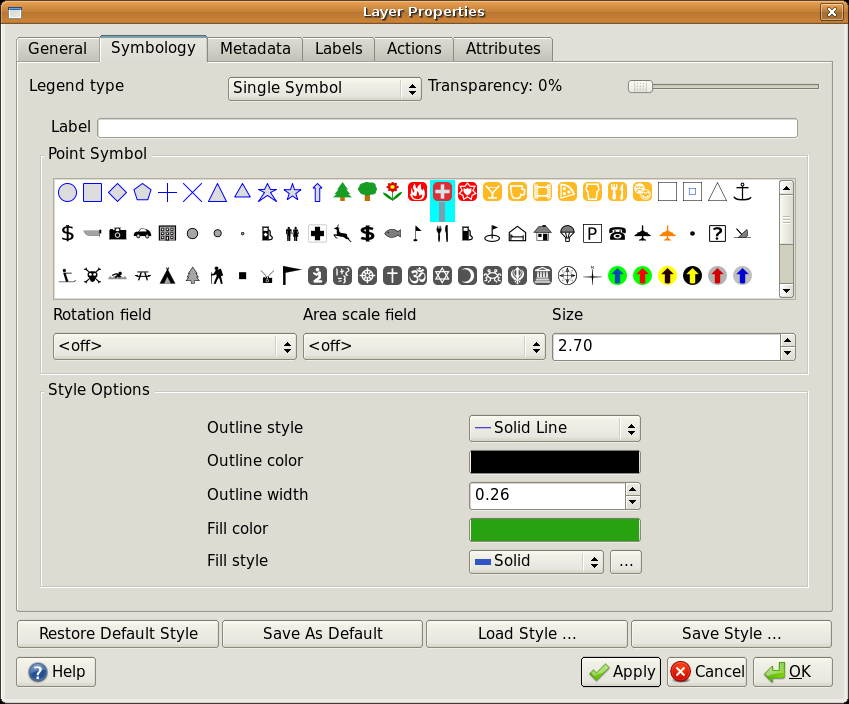
\includegraphics[clip=true, width=0.45\textwidth]{single_symbol_dialog_point}}\goodgap
   \subfigure[There are different options when defining simple symbols for
polyline and polygon features.]
    {\label{subfig:polsymbol}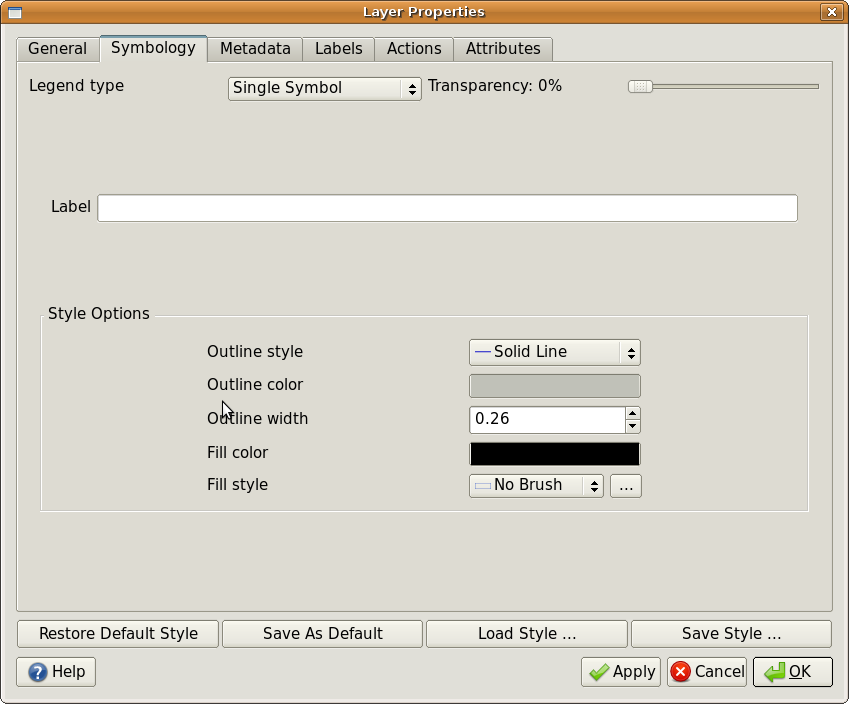
\includegraphics[clip=true, width=0.45\textwidth]{single_symbol_dialog_lines}}\goodgap
\end{figure}

\subsection{Graduated Symbols}

Sometimes vector features represent things with a changing numerical value.
Contour lines are a good example of this. Each contour usually has an
attribute value called 'height' that contains information about what height
that contour represents. In Figure \ref{fig:housesearch} earlier in this
topic we showed
contours all drawn with the same colour. Adding colour to the contours can
help us to interpret the meanings of contours. For example we can draw low
lying areas with one colour, mid-altitude areas with another and
high-altitude areas with a third.

%% Minipage to put both figures on one page
\begin{figure}[htpb]
   \begin{minipage}[h]{\textwidth}
   \begin{center}
   \caption{The height attribute of contours can be used to separate the
contours into 3 classes. Contours between 980m and 1120m will be drawn in
brown, those between 1120m and 1240m in green and those between 1240m and
1500m in purple.}
   \label{fig:gradcoldialog}\smallskip
   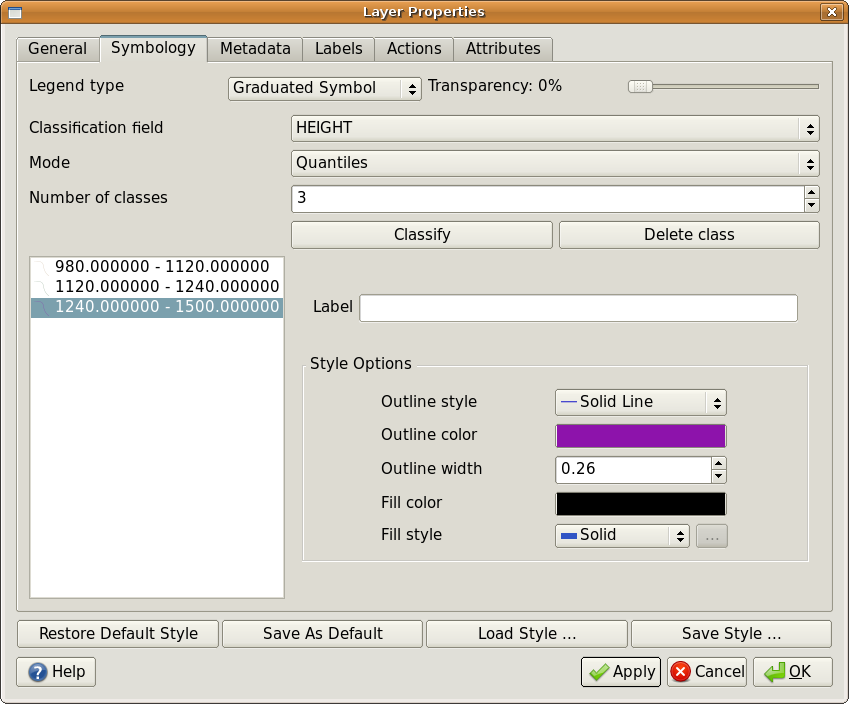
\includegraphics[clip=true, width=0.5\textwidth]{graduated_colour_dialog}
   \end{center}
   \end{minipage} \\
   \vspace{1cm}
   \begin{minipage}[h]{\textwidth}
   \begin{center}
   \caption{Our map after setting graduated colours for our contours.}
   \label{fig:gradcontours}\smallskip
   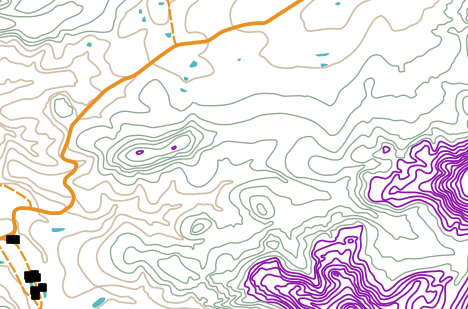
\includegraphics[clip=true, width=0.5\textwidth]{graduated_contours}
   \end{center}
   \end{minipage}
\end{figure}

Setting colours based on discrete groups of attribute values is called
Graduated Symbology in QGIS. The process is shown in Figure
\ref{fig:gradcoldialog} and \ref{fig:gradcontours}. \textbf{Graduated symbols
are most useful when you want to show clear
differences between features with attribute values in different value ranges}.
The GIS Application will analyse the attribute data (e.g. height) and, based
on the number of classes you request, create groupings for you. This process
is illustrated in Table \ref{tab:gradcolor}.

%% Define colors for the table
%% From http://oregonstate.edu/~peterseb/tex/samples/color-package.html
%% Note: xdvi does not show white text on black background but it works!
\begin{table}[ht]
\centering
\caption{Graduated colour breaks up the attribute value ranges into the
number of classes you select. Each class is represented by a different
colour.}\medskip
 \label{tab:gradcolor}
 \begin{tabular}{|p{8cm}|p{8cm}|}
 \hline
 \rowcolor{black}
 \textcolor{white}{\textbf{Attribute Value}} &
 \textcolor{white}{\textbf{Class and Colour}} \\
 \hline 1 & \colorbox{Apricot}{Class 1} \\
 \hline 2 & \colorbox{Apricot}{Class 1} \\
 \hline 3 & \colorbox{Apricot}{Class 1} \\
 \hline 4 & \colorbox{PineGreen}{Class 2} \\
 \hline 5 & \colorbox{PineGreen}{Class 2} \\
 \hline 6 & \colorbox{PineGreen}{Class 2} \\
 \hline 7 & \colorbox{Magenta}{Class 3} \\
 \hline 8 & \colorbox{Magenta}{Class 3} \\ 
 \hline 9 & \colorbox{Magenta}{Class 3} \\
\hline
\end{tabular}
\end{table}

\subsection{Continuous Colour Symbols}

In the previous section on Graduated Colour symbols we saw that we can draw
features in discrete groups or classes. Sometimes it is useful to draw
features in a \textbf{colour range} from one colour to another. The GIS Application
will use a numerical attribute value from a feature (e.g. contour heights or
pollution levels in a stream) to decide which colour to use. Table
\ref{tab:contcolor} shows how the attribute value is used to define a
continuous range of colours.

%% Define colors for the table !! not done yet !!
%% From http://oregonstate.edu/~peterseb/tex/samples/color-package.html
%% Note: xdvi does not show white text on black background but it works!
\begin{table}[ht]
\centering
\caption{Continuous colour symbology uses a start colour (e.g. light orange
shown here) and an end colour (e.g. dark brown shown here) and creates a
series of shades between those colours.}\medskip
 \label{tab:contcolor}
 \begin{tabular}{|p{8cm}|p{8cm}|}
 \hline
 \rowcolor{black}
 \textcolor{white}{\textbf{Attribute Value}} &
 \textcolor{white}{\textbf{Colour (no classes or grouping)}} \\
 \hline 1 & 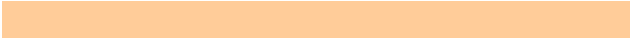
\includegraphics[width=7.5cm]{colorange1} \\
 \hline 2 & 
\includegraphics[width=7.5cm]{colorange2} \\
 \hline 3 & 
\includegraphics[width=7.5cm]{colorange3} \\
 \hline 4 & 
\includegraphics[width=7.5cm]{colorange4} \\
 \hline 5 & 
\includegraphics[width=7.5cm]{colorange5} \\
 \hline 6 & 
\includegraphics[width=7.5cm]{colbrown1} \\
 \hline 7 & 
\includegraphics[width=7.5cm]{colbrown2} \\
 \hline 8 & 
\includegraphics[width=7.5cm]{colbrown3} \\
 \hline 9 & 
\includegraphics[width=7.5cm]{colbrown4} \\
\hline
\end{tabular}
\end{table}

Using the same contours example we used in the previous section, let's see
how a map with continuous colour symbology is defined and looks. The process
starts by setting the layers properties to continuous colour using a dialog
like the one shown in Figure \ref{fig:contcoldialog}.

\begin{figure}[ht]
   \begin{center}
   \caption{Setting up continuous colour symbology. The contour height
attribute is used to determine colour values. Colours are defined for the
minimum and maximum values. The GIS Application will then create a gradient
of colours for drawing the features based on their heights.}
\label{fig:contcoldialog}\smallskip
   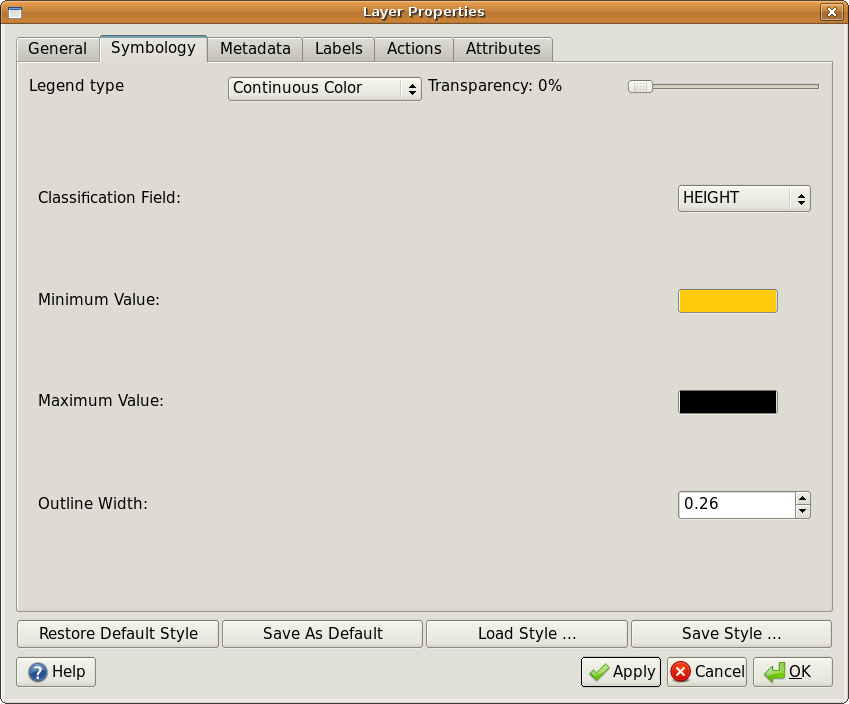
\includegraphics[clip=true, width=0.5\textwidth]{continuous_colour_dialog}
\end{center}
\end{figure}

After defining the minimum and maximum colours in the \textbf{colour range}, the
colour features are drawn in will depend on where the attribute lies in the
range between minimum and maximum. For example if you have contour features
with values starting at 1000m and ending at 1400m, the value range is 1000 to
1400. If the colour set for the minimum value is set to orange and the colour
for  the maximum value is black, contours with a value of close to 1400m will
be drawn close to black. On the other hand contours with a value near to
1000m will be drawn close to orange (see Figure \ref{fig:contourmap}).


\begin{figure}[ht]
   \begin{center}
   \caption{A contour map drawn using continuous colour symbology.}
\label{fig:contourmap}\smallskip
   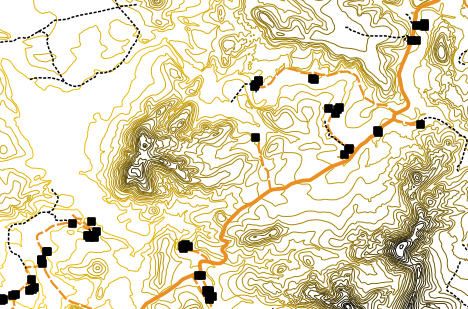
\includegraphics[clip=true, width=0.5\textwidth]{continuous_colour_contours}
\end{center}
\end{figure}

\subsection{Unique Value Symbols}

Sometimes the attributes of features are not numeric, but instead
\textbf{strings} are
used. 'String' is a computer term meaning a group of letters, numbers and
other writing symbols. Strings attributes are often used to classify things
by name. We can tell the GIS Application to give each unique string or number
its own colour and symbol. Road features may have different classes (e.g.
'street', 'secondary road', 'main road' etc.), each drawn in the map view of
the GIS with different colours or symbols. This is illustrated in Table
\ref{tab:unicolor}.

%% Note: xdvi does not show white text on black background but it works!
\begin{table}[ht]
\centering
\caption{Unique attribute values for a feature type (e.g. roads) can each
have their own symbol.}\medskip
 \label{tab:unicolor}
 \begin{tabular}{|p{8cm}|p{8cm}|}
 \hline
 \rowcolor{black}
 \textcolor{white}{\textbf{Attribute Value}} &
 \textcolor{white}{\textbf{Colour class and symbol}} \\
 \hline Arterial route & 
\includegraphics[width=7.5cm]{blueline} \\
 \hline Main road & 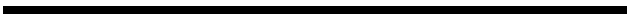
\includegraphics[width=7.5cm]{blackline} \\
 \hline Secondary road & 
\includegraphics[width=7.5cm]{apricotline} \\
 \hline Street & 
\includegraphics[width=7.5cm]{apricotdots} \\
\hline
\end{tabular}
\end{table}

Within the GIS Application we can open /choose to use Unique Value symbology
for a layer. The GIS will scan through all the different string values in the
attribute field and build a list of unique strings or numbers. Each unique
value can then be assigned a colour and style. This is shown in Figure
\ref{fig:univaldialog}.

\begin{figure}[ht]
   \begin{center}
   \caption{Defining unique value symbology for roads based on the road type.}
\label{fig:univaldialog}\smallskip
   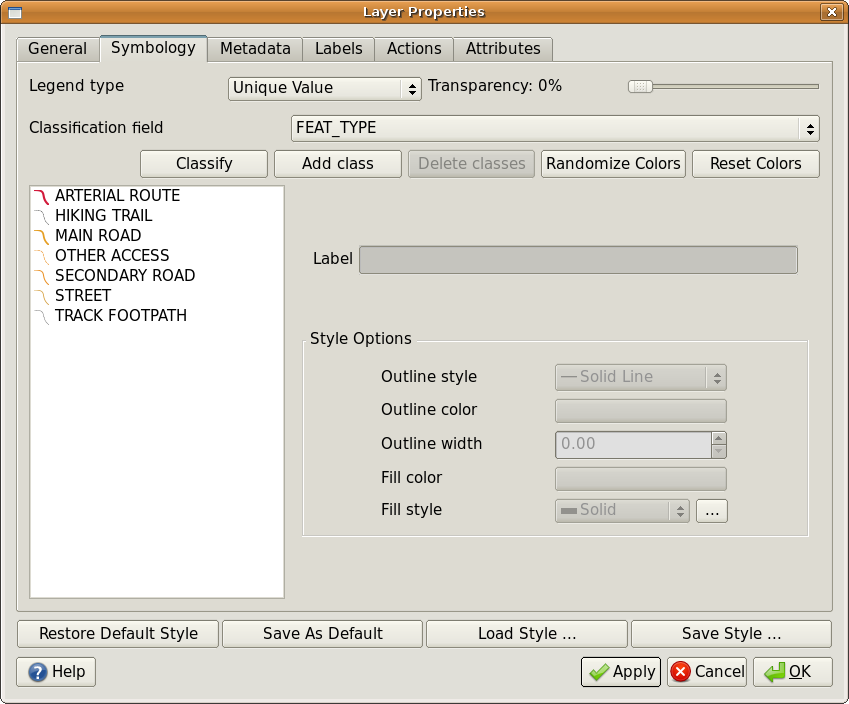
\includegraphics[clip=true, width=0.5\textwidth]{unique_value_dialog}
\end{center}
\end{figure}

When the GIS draws the layer, it will look at the attributes of each feature
before drawing it to the screen. Based on the value in the chosen field in
the attribute table, the road line will be drawn with suitable colour and
line style (and fill style if its a polygon feature). This is shown in
Figure \ref{fig:uniroads}.

\begin{figure}[ht]
   \begin{center}
   \caption{A roads vector layer symbolised using a unique value per road
type.}
\label{fig:uniroads}\smallskip
   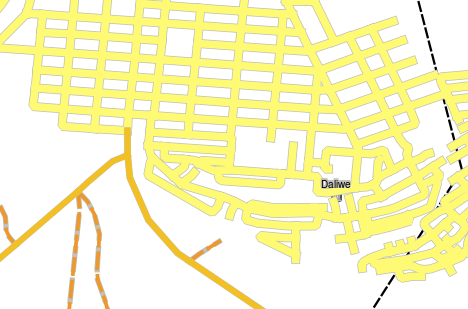
\includegraphics[clip=true, width=0.5\textwidth]{unique_value_roads}
\end{center}
\end{figure}

\subsection{Things to be aware of}

Deciding which attributes and symbology to use requires some planning. Before
you start collecting any \textbf{GeoSpatial} data, you should ensure you know what
attributes are needed and how it will be symbolised. It is very difficult to
go back and re-collect data if you plan poorly the first time around.
Remember also that the goal of collecting attribute data is to allow you to
analyse and interpret spatial information. How you do this depends on the
questions you are trying to answer. Symbology is a visual language that
allows people to see and understand your attribute data based on the colours
and symbols you use. Because of this you should put a lot of thought into how
you symbolise your maps in order to make them easy to understand.

\subsection{What have we learned?}

Let's wrap up what we covered in this worksheet:

\begin{itemize}
\item Vector features have \textbf{attributes}
\item Attributes \textbf{describe} the \textbf{properties} of the feature
\item The attributes are stored in a \textbf{table}
\item Rows in the table are called \textbf{records}
\item There is \textbf{one record per feature} in the vector layer
\item Columns in the table are called \textbf{fields}
\item Fields represent \textbf{properties} of the feature e.g. height, roof
colour etc.
\item Fields can contain \textbf{numerical}, \textbf{string} (any text) and
\textbf{date} information
\item The attribute data for a feature can be used to determine how it is
\textbf{symbolised}
\item \textbf{Graduated colour} symbology groups the data into discrete classes
\item \textbf{Continuous colour} symbology assigns colours from a colour
range to the features based on their attributes
\item \textbf{Unique value} symbology associates each different value in the
chosen attribute column with a different symbol (colour and style)
\item If the attribute of a vector layer is not used to determine its symbology, it
is drawn using a \textbf{single symbol} only
\end{itemize}

\subsection{Now you try!}

Here are some ideas for you to try with your learners:

\begin{itemize}
\item Using the table that you created in the last topic, add a new column for the
symbology type you would use for each feature type and have the learners
identify which symbology type they would use (see Table \ref{tab:featuretype}
for an example).
\item Try to identify which symbology types you would use for the following types
of vector features:
\begin{itemize}
\item points showing pH level of soil samples taken around your school
\item lines showing a road network in a city
\item polygons for houses with an attribute that shows whether it is made of brick,
wood or 'other' material.
\end{itemize}
\end{itemize}

%% Note: xdvi does not show white text on black background but it works!
\begin{table}[ht]
\centering
\caption{An example of a table that defines the feature types and the kind of
symbology you would use for each.}\medskip
 \label{tab:featuretype}
 \begin{tabular}{|p{4cm}|p{3cm}|p{9cm}|}
 \hline
 \rowcolor{black}
 \textcolor{white}{\textbf{Real world feature}} &
 \textcolor{white}{\textbf{Geometry Type}} & 
 \textcolor{white}{\textbf{Symbology Type}} \\
 \hline The school flagpole & Point & \textbf{Single Symbol} \\
 \hline The soccer field & Polygon & \textbf{Single Symbol} \\
 \hline The footpaths in and around the school & Polygon & Have your learners
count the number of learners using each footpath in the hour before school
and then use \textbf{graduated symbols} to show the popularity of each footpath \\
 \hline Places where taps are located & Point & \textbf{Single Symbol} \\
 \hline Classrooms & Polygon & \textbf{Unique Value} based on the grade of
the learners in the classroom \\
 \hline Fence & Polyline & Have your learners rate the condition of the fence
around your school by separating it into sections and grading each  section
on a scale of 1-9 based on its condition. Use \textbf{graduated symbols} to
classify the condition attribute. \\
 \hline Classrooms & Polygon & Count the number of learners in each classroom
and use a \textbf{continuous colour symbol} to define a range of colours from
red to blue. \\
\hline
\end{tabular}
\end{table}

\subsection{Something to think about}

If you don't have a computer available, you can use transparency sheets and a
1:50 000 map sheet to experiment with different symbology types. For example
place a transparency sheet over the map and using different coloured koki
pens, draw in red all contour lines below 900m (or similar) and in green all
lines above or equal to 900m. Can you think of how to reproduce other
symbology types using the same technique?

\subsection{Further reading}

\textbf{Website}: \url{http://en.wikipedia.org/wiki/Cartography#Map_symbology}

The QGIS User Guide also has more detailed information on working with
attribute data and symbology in QGIS.

\subsection{What's next?}

In the section that follows we will take a closer look at data capture. We
will put the things we have learned about vector data and attributes into
practice by creating new data.

